\chapter{Makefile and CMake}

\section{Large Project Structure}

When working on a large project, it is essential to organize your repository in a way that makes it easy to manage and understand. A typical structure might look like this:

\begin{itemize}
    \item \textbf{src/}: Contains all the source code files.
    \item \textbf{include/}: Contains all the header files.
    \item \textbf{lib/}: Contains external libraries.
    \item \textbf{build/}: Directory where the build system generates output files.
    \item \textbf{tests/}: Contains test code and test data.
    \item \textbf{docs/}: Contains documentation files.
    \item \textbf{CMakeLists.txt}: The main CMake configuration file.
    \item \textbf{README.md}: A file that provides an overview of the project.
\end{itemize}

This structure helps in maintaining a clean and organized codebase, making it easier for multiple developers to collaborate and for new developers to get up to speed quickly.

\begin{figure}[H]
    \centering 
    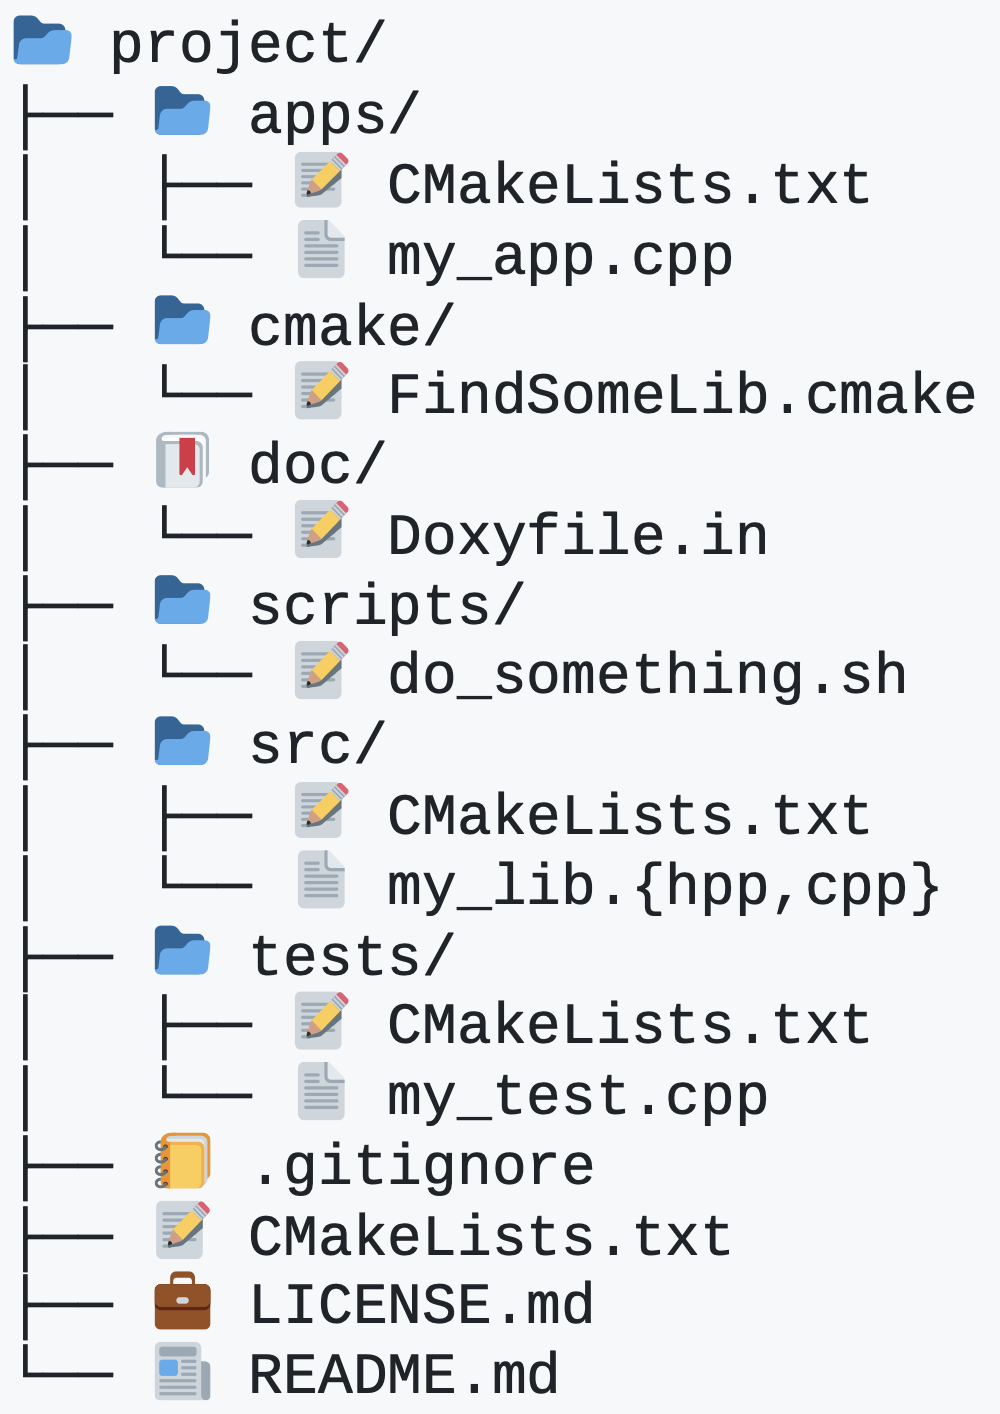
\includegraphics[width=0.4\textwidth]{assets/large_project.png}
    \caption{large Project Structure}
\end{figure}

\newpage
\section{Makefile}


A \texttt{Makefile} can automate compilation and linking processes for your project. make efficiently determines the need to regenerate a target by checking its existence and the up-
to-dateness of prerequisite files. This feature enables it to avoid unnecessary target regeneration.
Make simplifies the installation of numerous libraries through a concise set of commands. A typical
sequence for installing an open-source library involves using the following commands:

\begin{codeblock}[language=bash]
    make  ##builds the library
    make install   ##copies the library's headers, the libraries and the binaries to a user-specified folder
\end{codeblock}

\begin{itemize}
    \item \textbf{Target:} represents the desired output or action. It can be an executable, an
object file, or a specific action like "clean."
    \item \textbf{Prerequisites:} are files or conditions that a target depends on. If any of the prerequisites have
been modified more recently than the target, or if the target does not exist, the associated
recipe is executed.
    \item \textbf{Recipes:} is a set of shell commands that are executed to build or update the target.
\end{itemize}

Considering a very simple case where we only have three files (math.hpp, math.cpp and main.cpp), we can write:

\begin{codeblock}[language=bash]
main.o: main.cpp math.hpp   ## for compilation
    g++ std=c++17 -Wall main.cpp -c
math.o: math.cpp math.hpp   ## for compilation
    g++ -std=c++17 -Wall math.cpp -c
main: main.o math.o   ## for linking
    g++ main.o math.o -o main
clean:   ## for cleaning object files
    rm -rf main *.o
\end{codeblock}

A Makefile only redo the operations that contains files that have changed, and one can also call a single recipe instead of the entire file.


Use then variables for clarity and maintainability (used with \$(...))

\begin{codeblock}[language=bash]
CXX=g++
CPPFLAGS=-I.   ## for the preprocessor of either C++ or C
CXXFLAGS=-std=c++17 -Wall -Wpedantic -Werror   ## specific for c++ compiler

main.o: main.cpp math.hpp   ## for compilation
    $(CXX) $(CPPFLAGS) $(CXXFLAGS) main.cpp -c
math.o: math.cpp math.hpp   ## for compilation
    $(CXX) (CPPFLAGS) $(CXXFLAGS) math.cpp -c
main: main.o math.o   ## for linking
    $(CXX) $(CXXFLAGS) main.o math.o -o main
clean:   ## for cleaning object files
    rm -rf main *.o


###### since the first two commands are the same we can summarize the command

CXX=g++
CPPFLAGS=-I.   ## for the preprocessor of either C++ or C
CXXFLAGS=-std=c++17 -Wall -Wpedantic -Werror   ## specific for c++ compiler

all=main  ## convention used to specify the final target of the project

%.o: %.cpp math.hpp
    $(CXX) $(CPPFLAGS) $(CXXFLAGS) $< -c
main: $(OBJS)   ## for linking
    $(CXX) $(CXXFLAGS) $^$ -o $@
    ## $@ stands for the target file
    ## $^ expands to the list of all prerequisites (dependencies) of the current target
clean:   ## for cleaning object files
    rm -rf *.o

distcean:   ## convention to remove files generated during build process
    rm -rf main
\end{codeblock} 

Now we can introduce the dependencies:
\begin{codeblock}[language=bash]
    CXX=g++
CPPFLAGS=-I.   ## for the preprocessor of either C++ or C
CXXFLAGS=-std=c++17 -Wall -Wpedantic -Werror   ## specific for c++ compiler

DEPS=math.hpp
SRCS=$(wildcard *.cpp)  ##List of all .cpp files
OBJS=$(SRCS:.cpp=.o)  ##Same, but replace .cpp with .o

all=main  ## convention used to specify the final target of the project

%.o: %.cpp $(DEPS)
    $(CXX) $(CPPFLAGS) $(CXXFLAGS) $< -c
main: main.o math.o   ## for linking
    $(CXX) $(CXXFLAGS) $^$ -o $@
    ## $@ stands for the target file
    ## $^ expands to the list of all prerequisites (dependencies) of the current target
clean:   ## for cleaning object files
    rm -rf *.o

distcean:   ## convention to remove files generated during build process
    rm -rf main
\end{codeblock}

To use this \texttt{Makefile}, simply type:

\begin{codeblock}[language=bash][language=bash]
make
\end{codeblock}

To clean up:

\begin{codeblock}[language=bash][language=bash]
make clean
\end{codeblock}

Example with dynamic library:
\begin{codeblock}[language=bash]
    ### Library Makefile
    CXX=g++
    CPPFLAGS=-I.
    CXXFLAGS=-std=c++17 -Wall -Wpedantic -Werror
    
    SRC=$(wildcard *.cpp)
    OBJ=$(SRC:.cpp=.o)
    OBJ_fPIC=$(SRC:.cpp=.fpic.o)
    DEPS=$(wildcard *.h)
    
    LIB_NAME_SHARED=libparser.so
    
    all: shared 
    shared: $(LIB_NAME_SHARED)
    
    $(LIB_NAME_SHARED): $(OBJ_fPIC)
    	g++ $(CXXFLAGS) -shared $^ -o $@
    
    %.fpic.o: %.cpp $(DEPS)
    	$(CXX) -c -fPIC $(CPPFLAGS) $(CXXFLAGS) $^ -o $@
    
    %.o: %.cpp $(DEPS)
    	$(CXX) -c $(CPPFLAGS) $(CXXFLAGS) $^ -o $@
    
    clean:
    	rm -f *.o $(LIB_NAME_SHARED)
\end{codeblock}
\begin{codeblock}[language=bash]
    ### Project Makefile
    CXX=g++
    CPPFLAGS=-Iparser/
    CXXFLAGS=-std=c++17 -Wall -Wpedantic -Werror
    
    LDFLAGS=-Wl,-rpath,parser/ -Lparser/ # For dynamic linking.
    LDLIBS=-lparser # Link the shared library libparser.so
    
    SRC=ex1.cpp 
    OBJ=$(SRC:.cpp=.o)
    
    all: main
    
    main: $(OBJ)
    	$(CXX) $(CXXFLAGS) $^ $(LDFLAGS) $(LDLIBS) -o $@
    
    %.o: %.cpp
    	$(CXX) -c $(CPPFLAGS) $(CXXFLAGS) $< -o $@
    
    clean:
    	rm -f *.o main
\end{codeblock}
Then run in the terminal:
\begin{codeblock}[language=bash]
    ### In the library directory:
    make

    ### In the project directory:
    make

    ### Important thing is to insert the ex1.cpp in the project directory or update the directory in the Makefile
\end{codeblock}


\section{CMake}

\subsection*{Introduction}

CMake stands for "Cross-Platform Make." It is a \textbf{build-system generator}, meaning it creates the files (e.g., \texttt{Makefile}, Visual Studio project files) needed by your build system to compile and link your project.
CMake abstracts away platform-specific build configurations, making it easier to maintain code that needs to run on multiple platforms.

It works the following way:
\begin{enumerate}
    \item You write a \texttt{CMakeLists.txt} file that describes your project's configuration and structure.
    \item You run CMake on the \texttt{CMakeLists.txt} file to generate the build system files (e.g. \texttt{Makefile} on Linux or .snl for Visual Studio).
    \item You use the generated build system to compile and link your project.
\end{enumerate}

\subsection*{CMakeLists.txt}

Contains the configuration and structure of your project. It is a script that CMake uses to generate the build system files.
It has the following structure:

\begin{codeblock}[language=C++]
cmake_minimum_required(VERSION 3.10) 
project(MyProject)  

add_executable(my_project_main.cpp) 
\end{codeblock}

\subsubsection{Minimum Version}

Here is the first line of every \texttt{CMakeLists.txt}, which is the required name of the file CMake looks for:
\begin{codeblock}[language=bash]
cmake_minimum_required(VERSION 3.10)
\end{codeblock}
The version on CMake dictates the policies. Starting in CMake 3.12, this supports
a range like \texttt{3.12...3.15}. This is useful when you want to use new features but still support older versions.
\begin{codeblock}[language=bash]
cmake_minimum_required(VERSION 3.12...3.15)
\end{codeblock}

\subsubsection{Setting a project}
Every top-level CMake file will have this line:
\begin{codeblock}[language=C++]
project(MyProject VERSION 1.0
    DESCRIPTION "My Project"
    LANGUAGES CXX)
\end{codeblock}

Strings are quoted, whitespace does not matte and the name of the prokect is the first argument.
All the keywords are optional. The \texttt{version} sets a bunch of variables, like \texttt{MyProject\_VERSION} 
and \texttt{PROJECT\_VERSION}. The \texttt{LANGUAGES} keyword sets the languages that the project will use. This is useful for IDEs that support multiple languages.

\subsubsection{Making an executable}

\begin{codeblock}[language=C++]
add_executable(my_project_main my_project_main.cpp)
\end{codeblock}

\texttt{my\_project} is both the name of the executable file generate and the name of the CMake target created.
The source file comes next and you can add more than one source file. CMake will only compile source file extensions. 
The headers will be ignored for most purposes; they are there only to be showed up in IDEs.

\subsubsection{Making a library}

\begin{codeblock}[language=C++]
add_library(my_library STATIC my_library.cpp)
\end{codeblock}

\texttt{STATIC} is the type of library. It can be \texttt{SHARED} or \texttt{MODULE}. The source files are the same as for executables.
Often you'll need to make a fictional target, i.e., one where nothing needs to be compiled, for example for header-only libraries. This is called an \texttt{INTERFACE library},
and the only difference is that it cannot be followed by filenames.

\subsubsection{Targets}

Now we've specified a target, we can set properties on it.
CMake is all about targets and properties. An executable is a target, a library is a target. Your
application is built as a collection of targets depending on each other.


\begin{codeblock}[language=C++]
target_include_directories(my_library PUBLIC include)
\end{codeblock}

This sets the include directories for the target. The \texttt{PUBLIC} keyword means that the include directories will be propagated to any target that links to \texttt{my\_library}.
We can then chain targets:

\begin{codeblock}[language=C++]
add_library(my_library STATIC my_library.cpp)
target_link_libraries(my_project PUBLIC my_library)
\end{codeblock}

This will link \texttt{my\_project} to \texttt{my\_library}. The \texttt{PUBLIC} keyword means that the link will be propagated to any target that links to \texttt{my\_project}.

Targets can have include directories, linked libraries (or linked targets), compile options, compile definitions, 
compile features and more.

\subsubsection{Variables}

\texttt{Local variables} are used to store values that are used only in the current scope:

\begin{codeblock}[language=C++]
set(MY_VAR "some_file") 
\end{codeblock}

The names of the variables are case-sensitive and the values are strings. You access a variable by using \texttt{\$\{\}}.
CMake has the concept of scope; you cna access the value of the variable after you set it as long as you are in the same scope. If you leave a function or a file in a sub directory, the variable will 
no longer be defined. You can set a variable in the scope immediately above your current one with \texttt{PARENT\_SCOPE} at the end. 

One can also set a list of values:

\begin{codeblock}[language=C++]
set(MY_LIST "value1" "value2" "value3")
\end{codeblock}

which internally becomes a string with semicolons. You can access the values with \texttt{\$\{MY\_LIST\}}.

If you want to set a variable from the command line, CMake offers a variable cache.
\texttt{Cache variables} are used to interact with the command line:

\begin{codeblock}ì[language=C++]
set(MY_CACHE_VAR "VALUE" CACHE STRING "Description")

option(MY_OPTION "Set from command line" ON)
\end{codeblock}

Then:
\begin{codeblock}[language=bash]
cmake /path/to/src/ \
-DMY_CACHE_VAR="some_value" \
-DMY_OPTION=OFF
\end{codeblock}

\texttt{Environment variables} are used to interact with the environment:

\begin{codeblock}[language=bash]
# Read
message(STATUS $ENV{MY_ENV_VAR})

# Write
set(ENV{MY_ENV_VAR} "some_value")
    
\end{codeblock}

But it is not recommended to use environment variables in CMake.

\subsubsection{Properties}

The other way to set properties is to use the \texttt{set\_property} command:

\begin{codeblock}[language=C++]
set_property(TARGET my_library PROPERTY CXX_STANDARD 17)
\end{codeblock}

This is like a variable, but it is attached to a target. The \texttt{PROPERTY} keyword is optional. The \texttt{CXX\_STANDARD} is a property that sets the C++ standard for the target.